\chapter{Десорбция дейтерия из вольфрама при лазерном нагреве}\label{ch:ch4}

В настоящее время активно ведется разработка методов дистанционного контроля содержания изотопов водорода, которые основаны на взаимодействии лазерного излучения с поверхностью ОПЭ. Одним из таких перспективных подходов является лазерно-индуцированная десорбция (ЛИД). Этот метод включает в себя нагрев части поверхности с помощью лазерного импульса с последующим анализов вышедших частиц. Процедура ЛИД была успешно протестирована на нескольких токамаках, и сейчас ведется работа над созданием соответствующего комплекса для проекта ИТЭР~\cite{Zlobinski2024}. Ключевой задачей в этом процессе является определение оптимальных режимов работы, а также оценка возможных источников погрешности в измерениях.

Для применения в ЛИД рассматриваются лазерные системы с длительностью импульса вплоть до нескольких миллисекунд. Импульсный нагрев с большей длительностью позволяет проводить анализ содержания изотопов водорода на большей глубине~\cite{Yu2019, Zlobinski2020}, когда короткие импульсы (порядка наносекунд) позволяют исследовать тонкий поверхностный слой~\cite{Gasparyan2021}. Примечательно, что длительность на уровне миллисекунд сопоставима с длительностью импульсных нагрузок во время ELM-событий. С математической точки зрения, обе задачи весьма похожи, что позволяет проводить анализ в рамках одного подхода.  

Беря во внимание недавнее решение Международный организации ИТЭР о переходе к полностью вольфрамовой облицовке, актуальным вопросом является исследование ЛИД изотопов водорода из вольфрамовых слоев. Также необходимо напомнить, что в услоиях токамака основным каналом накопления изотопов водорода является соосаждение. Этот механизм приводит к образованию пленок на поверхности ОПЭ, теплофизические свойства которых могут отличаться от случая материалов с идеальной структурой. В данной главе на основе численного моделирования проводится анализ закономерностей выхода дейтерия из вольфрама при импульсном лазерном нагреве. Рассматривается влияние различных эффектов, связанных как с процессами на поверхности, так и с параметрами материала. Как и в прошлой главе, сначала перед представлением основных результатов моделирования в данной главе проводится оценка применимости используемого подхода основе сравнения с экспериментальными данными, полученными в экспериментах на КСПУ-Т~\cite{Poskakalov2020}. \fixme{Все исходные коды в программном пакете FESTIM и результаты проведенных расчетов также распространяются свободно. ССЫЛКА НА ГИТ И ЗЕНОДО}

\section{Моделирование эксперимента по ЛИД дейтерия и соосажденных пленок вольфрама}\label{sec:ch4/sec1}

\subsection{Детали эксперимента}\label{subsec:ch4/sec1/subsec1}

Эксперименты по ЛИД проводились на базе физико-технического института им. А. Ф. Иоффе. В них использовались пленки вольфрама, соосажденные с дейтерием. Пленки были нанесены на медные подложки ($20 \times 20 \times \SI{3}{\milli\metre}$) методом импульсного лазерного осаждения в атмосфере дейтерия (давление \SI{30}{\pascal}) с плазменным ассистированием при частоте \SI{13.56}{\mega\hertz}. Для осаждения плёнок вольфрама использовался твердотельный лазер Nd:YAG с длиной волны \SI{1064}{\nano\meter}, энергией в импульсе \SI{1.3}{\joule}, длительностью импульса \SI{12}{\nano\second} и частотой следования импульсов \SI{10}{\hertz}. Лазерное излучение фокусировалось на вольфрамовой мишени для обеспечения плотности энергии $\approx\SI{25}{\joule\per\centi\meter\squared}$. Осаждение проводилось в течение 15 минут при водяном (\SI{18}{\degreeCelsius}) охлаждении держателя подложки. Измеренная толщина осажденных пленок составила $\approx\SI{1}{\micro\metre}$.

Полученные образцы укладывались на медное основание ($100 \times 80 \times \SI{3}{\milli\metre}$). Для обеспечения лучшего теплоотвода во время ЛИД между медным основанием и образцами устанавливались индиевые прокладки. Композитная мишень фиксировалась медной рамкой с окошками, как показано на рисунке~\cref{fig:ch4/LID_target}. Образцы облучались лазерными импульсами с длительностью \SI{220}{\micro\second} и \SI{1}{\milli\second} (оптоволоконная лазерная система, IPG YLR-2000, \SI{1070}{\nano\metre}). Для ясности далее в работе первый случай будет относиться к микросекундному нагреву, а второй "--- к миллисекундному. Полная энергия лазерных импульсов варьировалась в диапазоне от \SI{0.12}{\joule} до \SI{0.35}{\joule} и от \SI{0.25}{\joule} до \SI{1.00}{\joule} для микросекундной (\( \SI{220}{\micro\second} \)) и миллисекундой (\(\SI{1}{\milli\second}\)) длительности импульса, соответственно. Анализ образцов после проведения ЛИД не показал явных изменений поверхности.

\begin{figure}[ht]
    \centerfloat{
        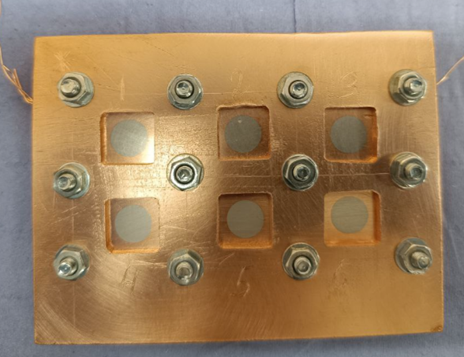
\includegraphics[scale=0.7]{LID_target.png}
    }
    \caption{Вид образцов с пленками вольфрама, расположенных на медном основании. Серые области "--- вольфрам-дейтериевые пленки}\label{fig:ch4/LID_target}
\end{figure}

Пространственный профиль плотности энергии измерялся лазерным анализатором SP620U OPHIR-SPIRICON. Полученный профиль соответствовал распределению Гаусса с усредненным значением полной ширины на уровне $1/e^2$ равным \(w=\SI{1}{\milli\metre}\) (удвоенное стандартное отклонение соответственно \SI{0.5}{\milli\meter}). Временные профили лазерного импульса измерялись кремниевым фотодиодом ФДУК-200 в фотогальваническом режиме. Временной профиль имели прямоугольную форму с характерной длительностью нарастания/затухания импульса равной \( \approx \SI{10}{\micro\second} \). Экспериментальный стенд для исследования ЛИД (см. рисунок~\ref{fig:ch4/LID_scheme}) включал в себя оптическую схему на основе двухлинзовой фокусирующей системы Галилея, систему перемещения лазерного луча по поверхности и вакуумный объём ($\approx\SI{70}{\liter}$). Вакуумный объём откачивался турбомолекулярным насосом (Turbovac 90i, Leybold) до базового уровня давления \SI{8e-5}{\pascal}. 

\begin{figure}[ht]
    \centerfloat{
        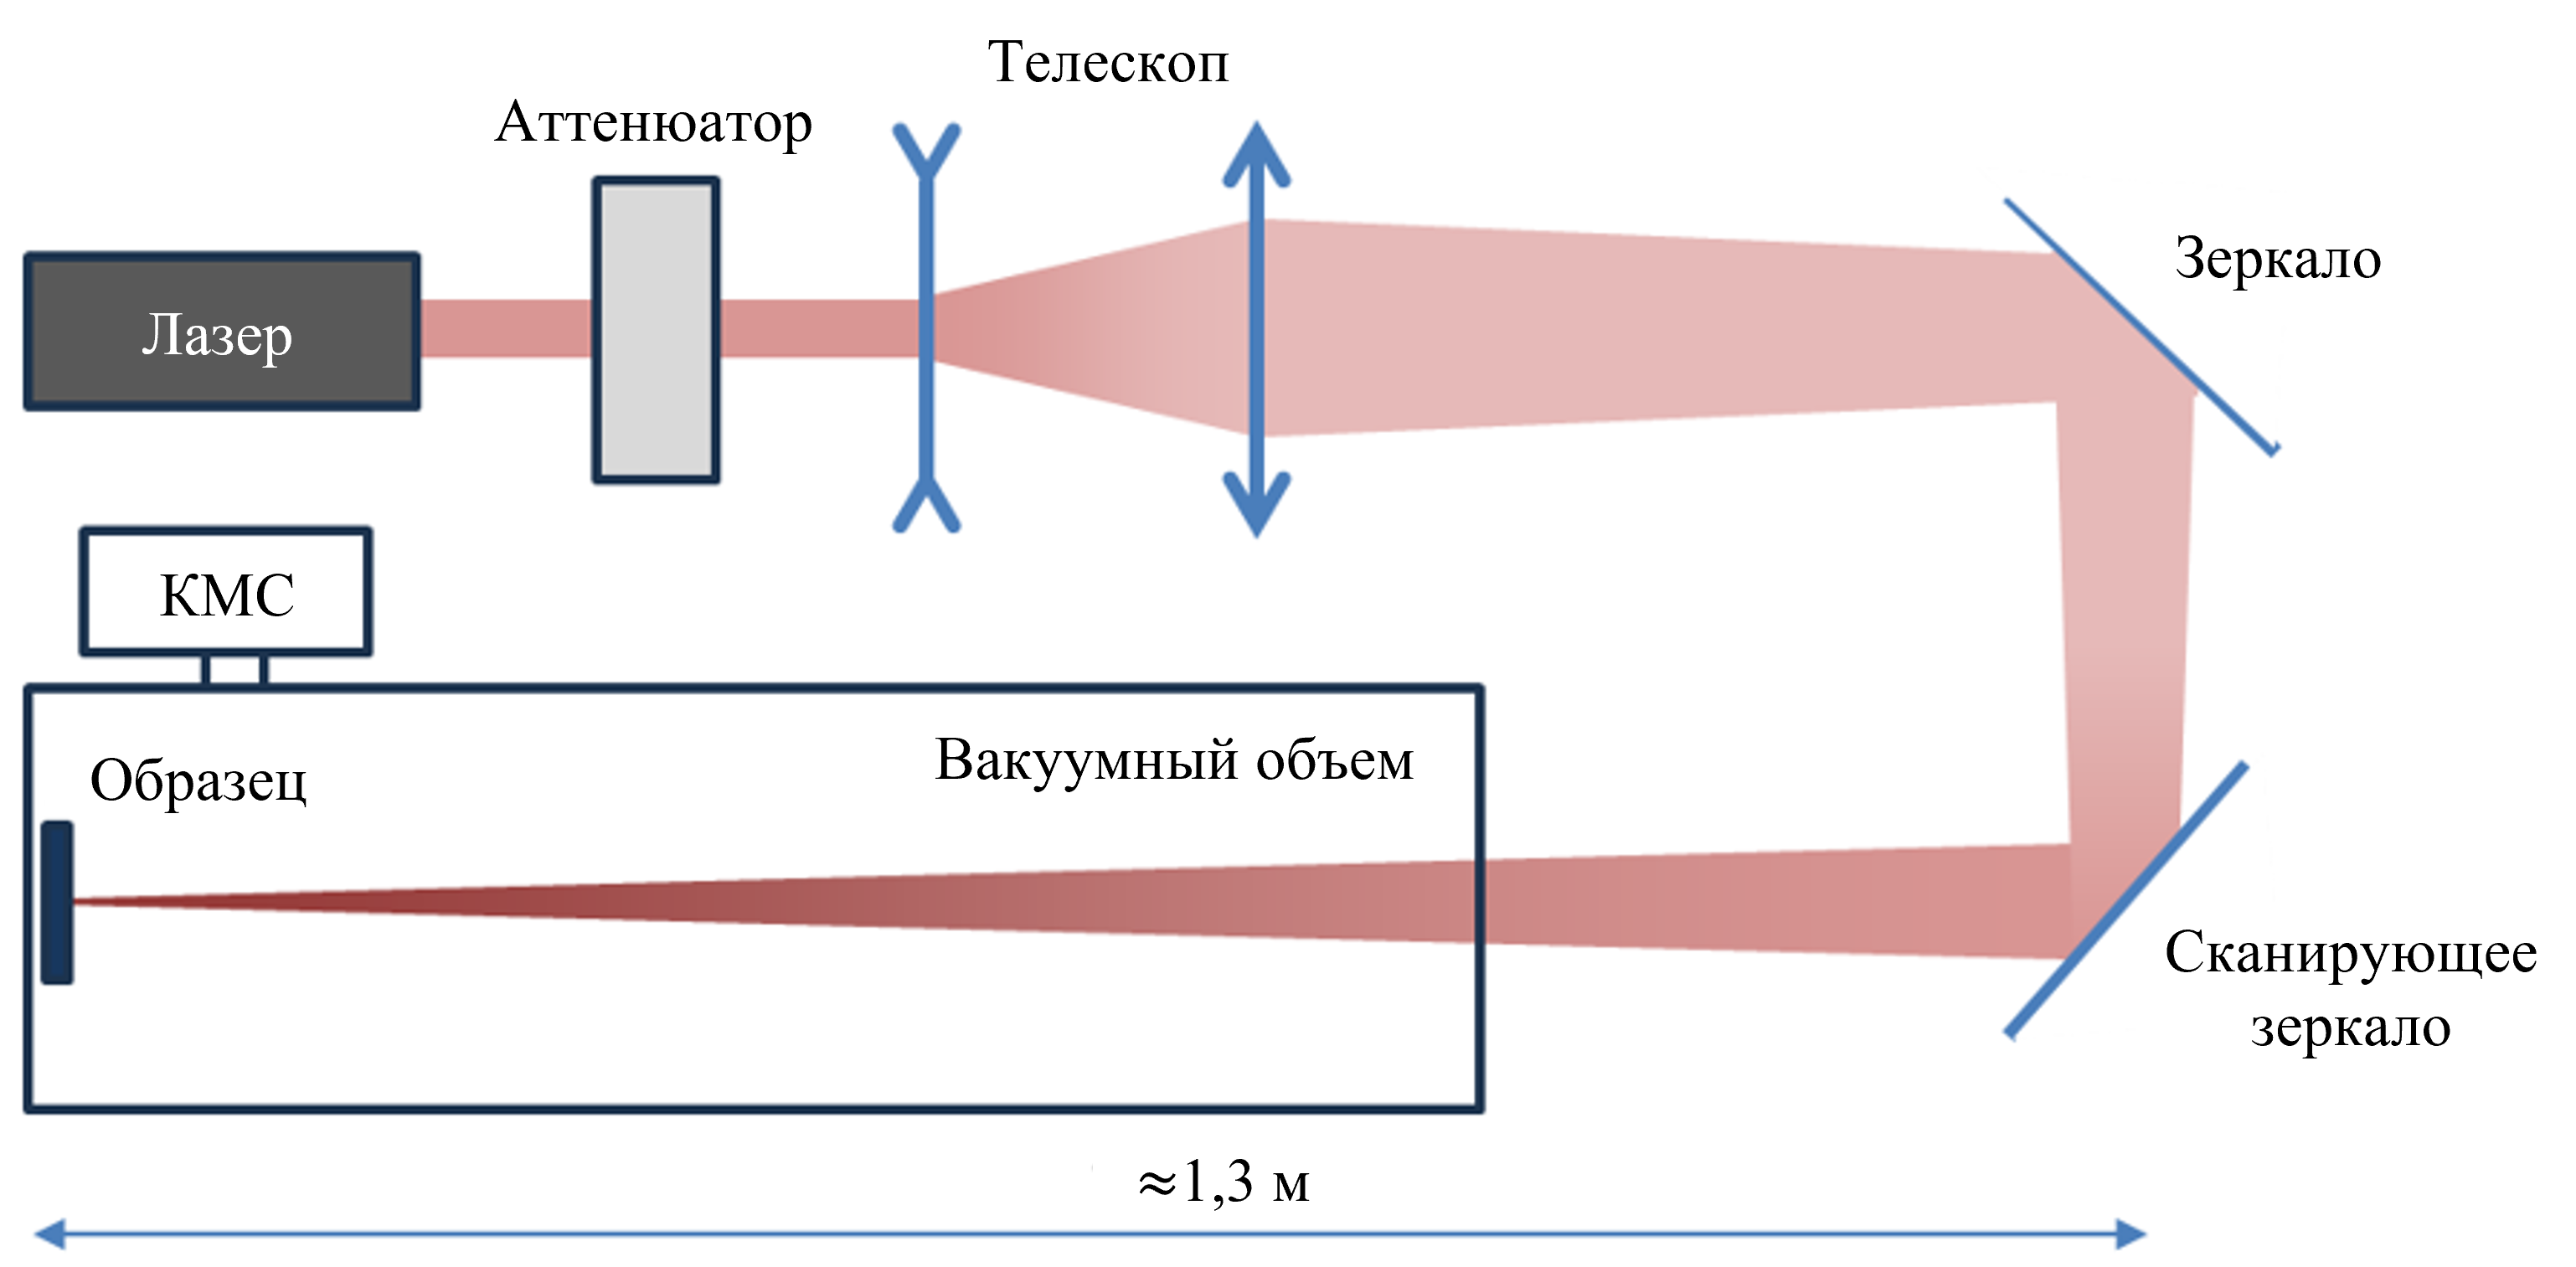
\includegraphics[scale=0.65]{LID_optic_scheme_ru.png}
    }
    \caption{Схема установки для проведения измерений ЛИД~\cite{Medvedev2024}}\label{fig:ch4/LID_scheme}
\end{figure}

Серия измерений при каждой длительности лазерного пучка проводились на отдельном образце. Участки поверхности образцов облучались серией импульсов с частотой \SI{0.1}{\hertz}. Регистрация сигналов 2; 3 и 4 масс проводилась с помощью КМС (Extorr XT300M). Масс-спектрометр калибровался по постоянному потоку дейтериевой течи с уровнем потока \SI{e-6}{\metre\cubed\pascal\per\second}. В ходе экспериментов изменения в сигналах 3 и 4 масс были ярко выражены, когда сигнал 2-ой массы не отличался от фонового. После серии импульсов энергия лазерного пучка и облучаемая область поверхности менялись. Смещение лазерного пятна происходило на такое расстояние, чтобы избежать влияния предыдущих импульсов на результаты измерений последующих. Для упрощения сравнения результатов численного моделирования с экспериментом из каждой серии импульсов при различных энергиях пучка использовались только первые выстрелы. Откалиброванный сигнал от первого выстрела интегрировался по времени для определения полного числа десорбированных атомов дейтерия. Температура поверхности образцов в ходе экспериментов не измерялась ввиду ограничений экспериментального стенда.

Получение дополнительной информации о параметрах центров захвата в осажденных пленках осуществлялось методом ТДС. Были исследованы аналогичные образца с соосажденными пленками, толщиной \SI{0.5}{\micro\metre}. Измерения проводились на сверхвысоковакуумном стенде \thesisOrganizationShort \ (кафедра №21)~\cite{Rusinov2009} с постоянной скоростью нагрева \SI{0.5}{\kelvin\per\second}. Сигналы десорбированных дейтерийсодержащих молекул регистрировались КМС (HIDEN), работающим с использованием метода пороговой ионизации. Калибровка масс-спектрометра проводилась в соответствии с процедурой, описанной в работе~\cite{Rusinov2009}. 

\subsection{Расчетная модель}\label{subsec:ch4/sec1/subsec3}

С целью воспроизведения результатов экспериментальных измерений ЛИД дейтерия из вольфрама была рассмотрена упрощенная геометрическая модель в цилиндрических координатах с аксиальной симметрией (см. рисунок~\cref{fig:ch4/LID_geom}), состоящая из двух материалов: вольфрамовой пленки (\SI{1}{\micro\meter}) и медной подложки (\SI{6}{\milli\meter}). Радиус расчетной области был выбран равным \SI{2}{\milli\meter}. На таком радиусе интенсивность лазерного импульса существенно затухает (в \( 1/e^{32} \) раз). Характерный масштаб распространения тепла за время лазерного воздействия с миллисекундной длительностью составляет \( L_\mathrm{heat}=\sqrt{\kappa \tau_\mathrm{ms}/C_p \rho} \approx \SI{0.2}{\milli\meter} \), что также не превышает величины радиального размера геометрической модели. 

\begin{figure}[ht]
    \centerfloat{
        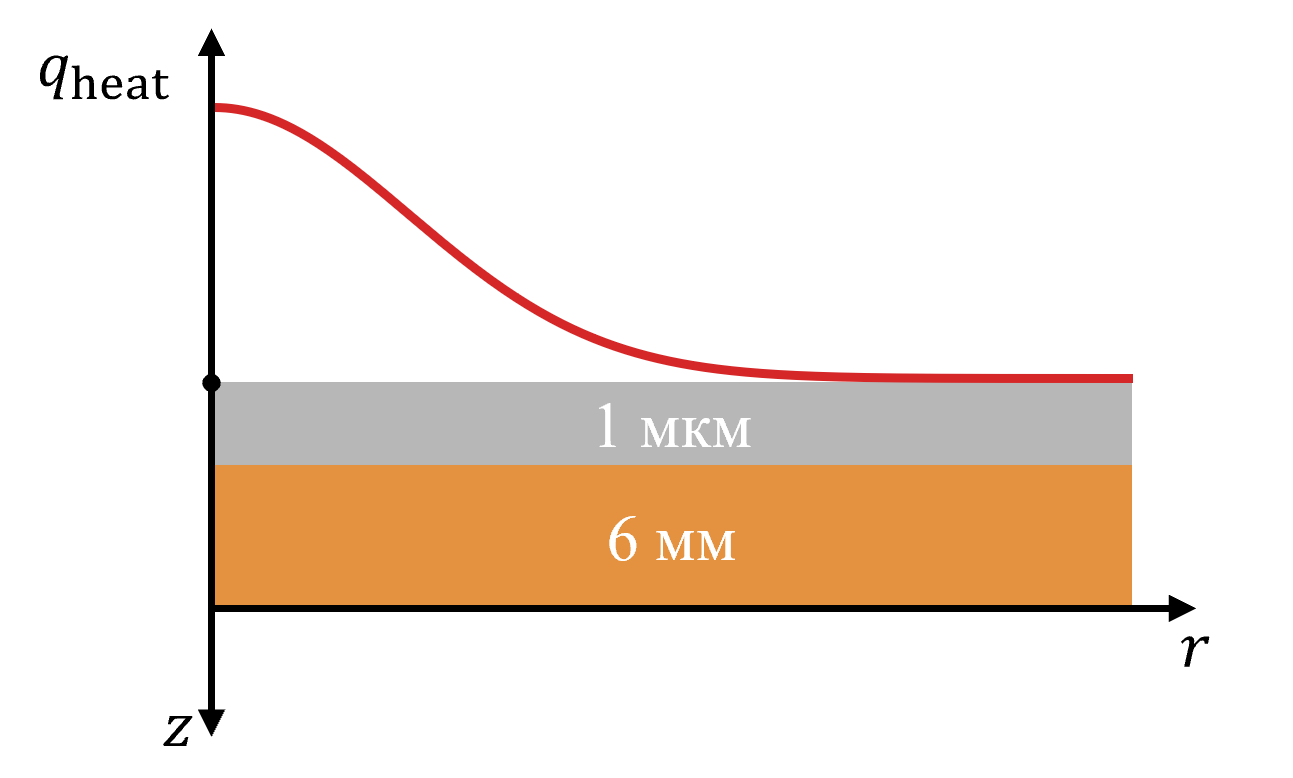
\includegraphics[scale=1]{LID_geom.png}
    }
    \caption{Схематическое представление двумерной геометрической модели, использованной при расчетах ЛИД. Радиус модели \SI{2}{\milli\meter}; \cruleme[customgrey]{0.5cm}{0.5cm}~---~W; \cruleme[customorange]{0.5cm}{0.5cm} "--- Cu.}\label{fig:ch4/LID_geom}
\end{figure}

Было рассмотрено однородное уравнение теплопроводности в приближении идеального теплового контакта между пленкой и подложкой: 
\begin{align}
    C_p \rho \frac{\partial T}{\partial t} = \frac{1}{r}\frac{\partial}{\partial r}\left( \kappa r \frac{\partial T}{\partial r} \right) + \frac{\partial }{\partial z}\left( \kappa \frac{\partial T}{\partial z} \right).
\end{align}
Температурная зависимость теплофизических свойств вольфрама и меди определялась уравнениями~\cref{eq:app/W_props,eq:app/Cu_props}. Нагрев за счет лазерного воздействия моделировался в качестве плотности мощности на границе:
\begin{equation}
    -\kappa \left. \frac{\partial T}{\partial z} \right\vert_{z=0} = q(r, t),
\end{equation}
Данное приближение справедливо, когда глубина проникновения лазерного излучения в твердое тело намного меньше характерного пространственного масштаба переноса тепла. Для вольфрама глубина проникновения излучения в ближнем инфракрасном диапазоне составляет величину \( \sim \SI{10}{\nano\meter} \)~\cite{Ordal1988}. Характерный масштаб переноса тепла при микросекундном нагреве можно оценить на уровне \( \sim \SI{0.1}{\milli\meter} \), что подтверждает справедливость приближения. Потерями мощности на излучение пренебрегается по сравнению с лазерным нагревом. Интенсивность лазерного импульса определялась на основе экспериментальных данных:
\begin{equation}
    q(r,t)=\frac{E_\mathrm{laser}}{2\pi \sigma_{r}^2\tau_\mathrm{imp}} \exp \left( -\frac{r^2}{2 \sigma_r^2} \right) \eta \left( \tau_\mathrm{imp}-t \right),
\end{equation}
где $E_\mathrm{laser}$ "--- полная энергия лазерного импульса, \si{\joule}; $\sigma_r=w/4=\SI{0.25}{\milli\meter}$ "--- стандартное отклонение пространственного распределения; \( \tau_\mathrm{imp} \) "--- длительность лазерного импульса, с; \(\eta(x)\) "--- функция Хевисайда. Передний/задний фронт во временной зависимости интенсивности лазерного импульса не учитывались. На остальных границах температура была фиксирована и равна начальной: \SI{300}{\kelvin}.

Задача транспорта дейтерия рассматривалась только для области вольфрама в силу того, что возможное проникновения дейтерия в медь не могло существенно влиять на сигнал измерений в режиме однократного облучения поверхности. Эволюция концентрации подвижных атомов дейтерия определялась из:
\begin{align}
    \frac{\partial \cm}{\partial t} = -\frac{1}{r}\frac{\partial (r J_r )}{\partial r} - \frac{\partial J_z}{\partial z} - \sum\limits_i \frac{\partial \cti}{\partial t},
\end{align}
где компоненты диффузионного потока определяются соответствующими компонентами градиентов концентрации и температуры. Процессы захвата и освобождения из дефектов определялись уравнением~\cref{eq:ch2/trapped_conc}. Полагалось, что все центры захвата распределены равномерно в слое вольфрама, что обычно справедливо для соосажденных пленок~\cite{Krat2020_2}. Начальная концентрация подвижных атомов была равна нулю, когда все дефекты считались полностью заполненными. На облучаемой поверхности задавалась нулевая концентрация подвижных атомов (приближение мгновенной десорбции), когда на остальных границах "--- нулевой поток. Параметры, определяющие транспорт дейтерия и сопутствующие процессы, приведены в таблице~\cref{tab:W_props}.

Определение параметров центров захвата (количество, концентрация, барьер освобождения) проводилось путем анализа ТДС-спектра на основе методики~\cite{Delaporte-Mathurin2021}, описанной ранее в настоящей работе. Моделирование проводилось в одномерном приближении. Температура было однородна по образцу и менялась линейно со временем. Параметры моделирования, граничные и начальные условия аналогичны тем, что использовались в задаче ЛИД. 

\subsection{Сравнение результатов моделирования и эксперимента}\label{subsec:ch4/sec1/subsec4}

На рисунке согласуется с результатами экспериментальных измерений (см. рисунок 6). 

\section{Анализ состава потока десорбированных частиц}\label{sec:ch4/sec2}
\subsection{Процессы на поверхности}\label{subsec:ch4/seс2/subsec1}

\begin{subequations}
    \begin{align}
        \frac{d \csurf}{dt} & = \Jbs - \Jsb + \Jvs, \\ 
        \lambda_\mathrm{abs} \frac{\partial \cm}{\partial t} & = -J + \Jsb - \Jbs + \Jvb.
    \end{align}
\end{subequations}

\subsection{Аналитический анализ}\label{subsec:ch4/seс2/subsec2}
\subsection{Результаты численного моделирования}\label{subsec:ch4/seс2/subsec3}

В настоящем исследовании эффективность LID определяется как доля атомов, десорбированных после одного теплового импульса (    ∕ 0). Количество десорбированных атомов сильно зависит от параметров лазерного импульса. В основном, импульсные нагрузки с более высокой плотностью мощности соответствуют более высоким температурам материала. Нагрев до более высоких температур и поддержание материала при таких температурах в течение более длительного времени делают высвобождение H более вероятным [47]. Было показано, что пиковая температура поверхности является важным параметром для характеристики шероховатости поверхности PFC, развивающейся после воздействия кратковременных тепловых нагрузок [58,59]. Таким же образом можно оценить эффективность ЛИД, измерив максимальную температуру образца, достигнутую при нагревании

\section{Анализ влияния параметров материала на выход дейтерия}\label{sec:ch4/seс3}
\subsection{Влияние теплопроводности материала}\label{subsec:ch4/seс3/subsec1}
\subsection{Влияние параметров центров захвата}\label{subsec:ch4/seс3/subsec2}
\subsection{Режимы десорбции во время лазерно-индуцированной десорбции}\label{sec:ch4/seс3/subsec3}

\section{Выводы к Главе~\ref{ch:ch4}}

\clearpage
